%!TEX root = ../main.tex
\begin{frame}{The Optimal Control Problem}
    \setlength{\leftmargini}{1mm}
    \begin{textblock*}{130mm}(3mm, 20mm)
        \only<1>{

            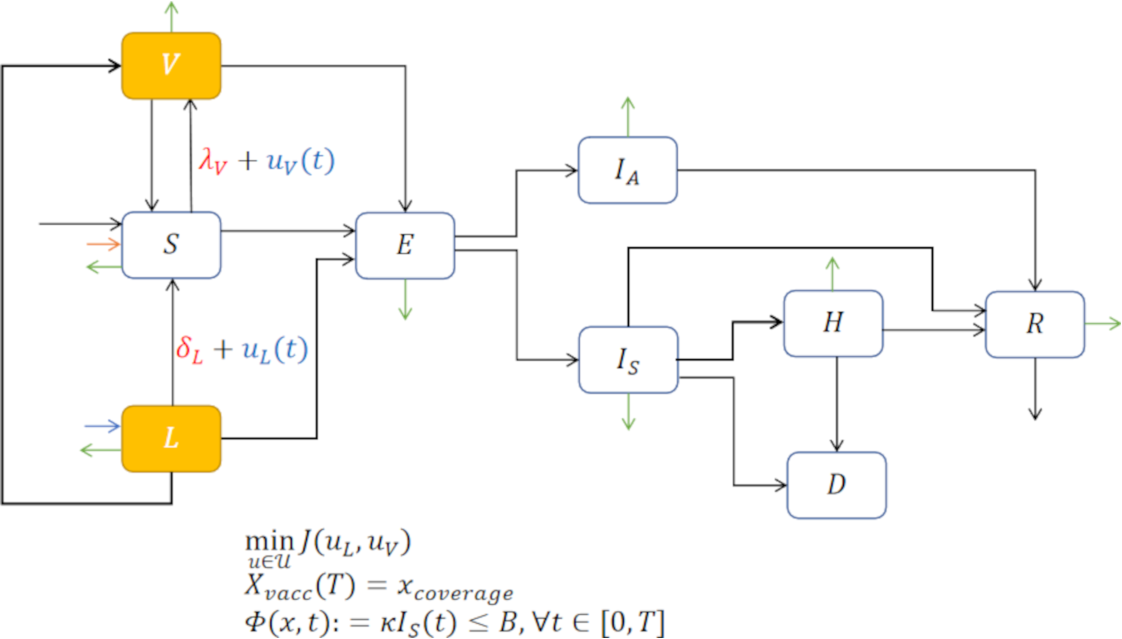
\includegraphics[scale=.65,%
                keepaspectratio]{assets/ControlledSchemes/lockdown_vaccination_controlled_scheme.pdf}
        }
    \end{textblock*}
\end{frame}
\begin{frame}{The disability-adjusted life year (DALY)}
    \begin{textblock*}{120mm}(5mm,7mm)
        %
        \begin{graybox}{{$DALY(c,s,a,t) = YLL(c,s,a,t) + YLD(c,s,a,t)$}}
            For given cause c, age a, sex s and year t
            \begin{description}
                \item[$YLL:$] Years of life lost due to premature death.
                    $$
                        YLL(c,s,a,t) = N(c,s,a,t) \times L(s,a)
                    $$
                    \begin{itemize}
                         \item
                             $N(c,s,a,t):$ is the number of 
                             deaths due to the cause $c$ 
                         \item
                             $L(s,a):$ is a standard loss 
                             function specifying years of life lost 
                    \end{itemize}
                 \item[$YLD:$] Years of life list due to disability   
                     $$
                         YLD(c,s,a,t) = I(c,s,a,t) \times DW(c,s,a) 
                         \times L(c,s,a,t)
                     $$
                    \begin{itemize}
                        \item
                            $I(c,s,a,t):$ number of incident cases for cause c
                        \item
                            $DW(c,s,a):$ disability weight for cause c
                        \item
                            $L(c,s,a,t):$  average duration of the case 
                            until remission or death (years)
                    \end{itemize}
            \end{description}
       \end{graybox}        
    \end{textblock*}

    \begin{textblock*}{120mm}(0mm,74mm)
       \begin{equation*}
            \begin{aligned}
             \only<2->{\min_{u_V  \in \mathcal{U}[0, T]}}
             J(u_V) := &
             \only<3->{
                \int_{0}^T
                    \underbrace{
                        a_S p \kappa E(r) 
                        +
                        a_H \delta_H I_s(r)
                    }_{:=YLL}
                    +
                    \underbrace{a_D
                        \left[
                            \mu_{I_S} I_S(r) + \mu_H H(r)
                        \right]}_{:=YLD}
                dr
            }
            \only<4->{
                +
                \\
                &
                \int_0^T
                    \frac{1}{2}
                    \left[
                        c_L u_L^2(r) +
                        c_V u_v^2(r)
                    \right]
                    dr.
            }
            \end{aligned}
       \end{equation*}
    \end{textblock*}

    \end{frame}
    %
    %
    \begin{frame}{Optimal Control Problem}
    \begin{textblock*}{120mm}(4mm,10mm)
        \only<1-3>{
            \begin{equation*}
                    \begin{aligned}
                             %
                             \textcolor<1>{orange}{%
                                \min_{u_V  \in \mathcal{U}[0, T]}
                                J(u_V) :=
                            }
                                 &
                                     \int_{0}^T
                                        \underbrace{
                                            a_S p \kappa E(r) 
                                            +
                                            a_H \delta_H I_s(r)
                                        }_{:=YLL}
                                        +
                                        \underbrace{a_D
                                        \left[
                                            \mu_{I_S} I_S(r) + \mu_H H(r)
                                        \right]}_{:=YLD}
                                    dr                         
                                    +
                                \\
                                    &
                                    \int_0^T
                                        \frac{1}{2}
                                        \left[
                                            c_L u_L^2(r) +
                                            c_V u_V^2(r)
                                        \right]
                                        dr
                        \\ 
                             \textcolor<2>{orange}{
                                u_V(\cdot)   \in [u_{\min}, u^{\max}],
                            }
                            &
                        \\
                            \textcolor<3>{orange}{
                                \kappa I_S(t)  
                                \leq B, \quad \forall t \in [0, T],
                             }
                             &
                    \end{aligned}
            \end{equation*}
        }
    \end{textblock*}    
    \begin{textblock*}{75mm}(2mm, 5mm)        
        \only<4->{
            \begin{equation*}
                \begin{aligned}
                    &\min_{u_V  \in \mathcal{U}[0, T]}
                    J(u_V) :=
                         \int_{0}^T
                            \underbrace{
                                a_S p \kappa E(r) 
                                +
                                a_H \delta_H I_s(r)
                            }_{:=YLL}
                            +
                            \underbrace{a_D
                            \left[
                                \mu_{I_S} I_S(r) + \mu_H H(r)
                            \right]}_{:=YLD}
                        dr                         
                        +
                    \\
                        &
                        \int_0^T
                            \frac{1}{2}
                            \left[
                                c_L u_L^2(r) +
                                c_V u_V^2(r)
                            \right]
                            dr
                    \\
                    \text{s.t.} &
                    \\
                        L' & =  \theta \mu N^{\star}
                            -\epsilon \lambda L - (u_L(t) + \delta_L) L - \mu L
                    \\
                        S' & =
                            (1 - \theta) \mu N^\star
                            + (u_L(t) + \delta_L) L
                            + \delta_V V
                    \\
                        & 
                            \qquad+ \delta_R R 
                            -
                            \left[
                                \lambda + (\lambda_V + u_V(t)) + \mu
                            \right] S
                    \\
                        E' &=
                            \lambda (\epsilon L + (1-\varepsilon) V + S)
                            - (\kappa + \mu) E
                    \\
                        I_S' &=
                            p \kappa E
                        - (\gamma_S +
                            \mu_{I_S} +
                            \delta_H +
                            \mu) I_S
                    \\
                        I_A' &=
                            (1 - p) \kappa E - (\gamma_A + \mu) I_A
                    \\
                        H' &=
                            \delta_H I_S - (\gamma_H + \mu_H + \mu) H
                    \\
                        R'  &=
                            \gamma_S I_S +
                            \gamma_A I_A +
                            \gamma_H H % +
                            - (\delta_R + \mu) R
                    \\
                        D' &=
                            \mu_{I_S} I_S + \mu_H H
                    \\
                        V' &=
                            (\lambda_V + u_V(t)) S
                    \\
                            &
                                - \left[
                                        (1 - \varepsilon) \lambda
                                    + \delta_V
                                    + \mu
                                \right ] V
                \end{aligned}
            \end{equation*}
        }
    \end{textblock*}
%
    \begin{textblock*}{60mm}(57mm, 30mm)
        \only<4->{
            \begin{equation*}
                \begin{aligned}
                    \frac{dX_{vac}}{dt}
                        &=
                        (u_V(t) + \lambda_V)
                        \left[
                            L + S + E + I_A + R
                        \right]
                \\
                    \frac{d Y_{I_S}}{dt}
                        & = p \kappa E
                \\
                \lambda &:=
                    \frac{\beta_A I_A + \beta_S I_S}{N^{\star}}
                \\
                \\
                L(0) &= L_0,
                \ S(0) = S_0,
                \ E(0) = E_0,
                \ I_S(0) = I_{S_{0}},
                \\
                I_A(0) &= I_{A_{0}},
                H(0) = H_0, \
                \ R(0) = R_0, \ D(0) = D_0,
                \\
                V(0) &= 0, \ X_{vac}(0) = 0, \quad
                u_V(.) \in [u_{\min}, u^{\max}],
                \\
                X_{vac}(T) &= x_{coverage},
                \quad
                \kappa I_S(t) \leq B, \qquad
                \forall t \in [0, T],
                \\
                N^{\star}(t) &=
                    L + S +E + I_S + I_A 
                \\
                   &
                    +
                    H + R + V
                \end{aligned}
            \end{equation*}
        }
    \end{textblock*}
\end{frame}